\section{Popup Graph}
Given the input image, either a vector image or a scalar image, we first segment the image. For a vector image, we read the segment information from the image directly. For a scalar image, we segment the image using Watershed algorithm. With the image segmentation, we then extract a family of popup graphs, each of which defines a specific popup design with unique configuration of fold lines and cuts. The common attribute of the family is derived from the input segmentation, and our goal to choose the best one from the family based on appealing popup properties. In this section, we will define popup graph, its family and how we build such a family from the input segmentation.

From the example in Figure \ref{fig:example} we can see, a popup design contains fold lines, cuts and patches. Multiple patches consist of an input segment and they are separately by fold lines. Cuts and fold lines form segment boundaries. So once the fold lines are given, we can acquire patch information by cutting segments with fold lines and retrieve cut information by looking at segment boundary. So with input segmentation, fold lines are the only information we need to define a popup design. A popup graph is thus defined by fold line properties.

Fold lines are vertical lines on the image domain, which either connect two segments or cut a segment through. Use $(u, v)$ to represent the image coordinate, two end points of a fold line $f$ are $(u(f), v_1(f))$ and $(u(f), v_2(f))$. So $u(f)$ is a key attribute we want to optimize. But instead of optimizing $v_1(f)$ and $v_2(f)$, we seek to pre-define a unique mapping between $u(f)$ and $(v_1(f), v_2(f))$ pair for each fold line so that, we can read out $v_1(f)$ and $v_2(f)$ based on $u(f)$. The unique mapping property holds once we specify a range for a fold line (see Figure \ref{fig:fold_line_mapping}). To ensure the completeness of solution space, we find all possible fold lines and introduce a variable $a(f)$ for fold line $f$ to indicate whether it is active or not. Besides $u(f)$ and $a(f)$, we add $c(f)$ to indicate the convexity of a fold line (whether it points outwards or inwards). We will explain how to find all fold line candidates and define their image-specific attributes including the unique mapping between $u(f)$ and $(v_1(f), v_2(f))$ pair. A popup graph $G$ is a graph of fold lines with a specific configuration of $u(f)$, $a(f)$, and $c(f)$ together with image-specific attributes. A popup graph family $\mathcal{G}$ is a family of popup graphs with common image-specific attributes (i.e. popup graphs derived from the same image).
% We define two types of popup graphs based on three types of units: \textit{segments}, \textit{regions}, and \textit{fold line candidates}. \textit{Segments} come directly from input image segmentation. Inside each segment, there are usually multiple \textit{regions}, each of which contains one fold line candidate. A fold line candidate is potentially effective fold line in the final design. There are two types of \textit{fold line candidates}. \textit{Intersection fold line candidates} come the intersection between two neighboring \textit{segment}. And \textit{region fold line candidates} come from each region. We first segment the input image (see section \ref{image_segmentation}), then find \textit{intersection fold line candidates} (see section \ref{intersection_fold_line_candidates}), and then find \textit{regions} and corresponding \textit{region fold line candidates} (see section \ref{region_fold_line_candidates}. We incorporate all information to build two types of graphs as explained in \ref{popup_graph_structure}.  Three units and two popup graphs are illustrated in Figure \ref{fig:graph}.

\subsection{Intersection Fold Lines Candidates} \label{intersection_fold_line_candidates}
We call a fold line which connects two segments as an ``intersection fold line''. For any given pair of neighboring segments, there could be an arbitrary number of fold lines with arbitrary position along the intersection. Ideally, we want one fold line candidate for each possible position, but then the optimization becomes intractable. In practice, we first divide the intersection into multiple parts such that each part is supposed to contain only one fold line and there exists unique mapping between $u(f)$ and $(v_1(f), v_2(f))$ pair. For this purpose, we define a \textit{slope} as a part of the intersection where $x$ is monotonically increasing or decreasing over $y$ as shown in Figure \ref{fig:valley}. Then we assign one fold line candidate for each \textit{slope}. Note that the fold line can appear at any location at the slope, but we use the location with the highest feasibility score as the default location for the fold line.
% We find that there is usually at most one fold line in each \textit{slope}. But dividing directly by \textit{slopes}, we borrow the idea of max-suppression. We first pick the position with the best score (defined below) and then suppress positions in the same slope (in cases where the picked position is at the intersection point of two slopes, positions in both slopes will be suppressed). We repeat the process for the remaining positions until are positions are considered. Each picked position will be the desirable position for one fold line candidate and corresponding suppressed positions will be the possible positions for this candidate.

% For a popup craft, fold lines serve as joints connecting two patches. Most fold lines lie between two neighboring segments and connect them. For any given pair of neighboring fold lines, there could be arbitrary number of fold lines with arbitrary position along the intersection. Ideally, we want one fold line candidate for each possible position, but then the optimization becomes intractable. The opposite extreme is to have only one fold line candidate but allows it to appear anywhere along the intersection. In practice, we first divide the intersection into multiple parts such that it is unlikely for each part to contain more than one fold lines. Then we assign one fold line candidate for each part. We define a \textit{slope} as a part of the intersection where $x$ is monotonically increasing or decreasing over $y$ as shown in Figure \ref{fig:valley}. We find that there is usually at most one fold line in each \textit{slope}. But dividing directly by \textit{slopes}, we borrow the idea of max-suppression. We first pick the position with the best score (defined below) and then suppress positions in the same slope (in cases where the picked position is at the intersection point of two slopes, positions in both slopes will be suppressed). We repeat the process for the remaining positions until are positions are considered. Each picked position will be the desirable position for one fold line candidate and corresponding suppressed positions will be the possible positions for this candidate.

To define the feasibility score for a fold line candidate at given position, we look at a local window around that position. The size of the window has clear physical meanings. When we make actual popup crafts out of a hard paper, a fold line has to be long enough so that it connects two patch stably. Also, we want patches beside it to be wide enough so that the fold line is easy to fold by hand. The height of the local window is chosen to be the minimal fold line length and the width of the local window is chosen to be twice of the minimal patch width beside a fold line. For a fold line $f$ to appear at pixel $p$, denote its left segment as $s_l$ and its right segment as $s_r$, the score of the fold line $f$, is determined as \ref{equ:goodness}.
\begin{equation}
  S(f, p, s_l, s_r) = \frac{|W_l(p) \cap R(s_l)| * |W_r(p) \cap R(s_r)|}{(0.5 H^f W^f)^2}
  \label{equ:goodness}
\end{equation}

% There are two key parameters in this task. $H^f$ is the desirable height of the local window of a fold line and $W^f$ is the desirable width of the local window. Here, the local window is simply a rectangle region on the image. For a pixel $p$ in $\mathcal{S}$, we look at its local window $W(p)$ with height $H^f$ and width $W^f$. There could be more than one segments $W(p)$ and for each pair of them which are adjacent, we can put a fold line between them at $p$. For any such pair, there are two options in terms of which one is left (right). For each option, denote the left segment as $s_l$ and the right segment as $s_r$, the score of the fold line $f$ between them at $p$ is determined as \ref{equ:goodness}.
% \begin{equation}
%   S(f, p, s_l, s_r) = \frac{|W_l(p) \cap R(s_l)| * |W_r(p) \cap R(s_r)|}{(0.5 H^f W^f)^2}
%   \label{equ:goodness}
% \end{equation}
% Here $W_l(p)$ and $W_(p)$ are the left half and right half of $W(p)$ respectively, and $R(s)$ is the region of $s$ on the image domain. The intuition for this equation is for a fold line to be more reliable, it should have more left segment pixels on its left and more right segment pixels on its right. The score is in $[0, 1]$ by its definition.

% After we iterated over all pixels and found all such fold line candidates, we use a greedy strategy to filter out the ones with lower score. In filtering process has two stages. In the first stage, the competition is among fold lines between same pair of segments with same direction. For each pair of segments with same direction, we first collect all the fold lines between them and corresponding pixels. We first choose to keep the one with the highest score, and then filter our all the fold lines which can be reached by going either to left or right along the segment boundary starting from the center point of this fold line. We repeat this process for remaining fold lines until all fold lines are considered. The intuition is to choose one fold line with the highest score in each ``valley'' (a ``valley'' is defined vertically on the boundary between this two segments). (See figure \ref{fig:valley}.)

% \begin{figure}[h]
%   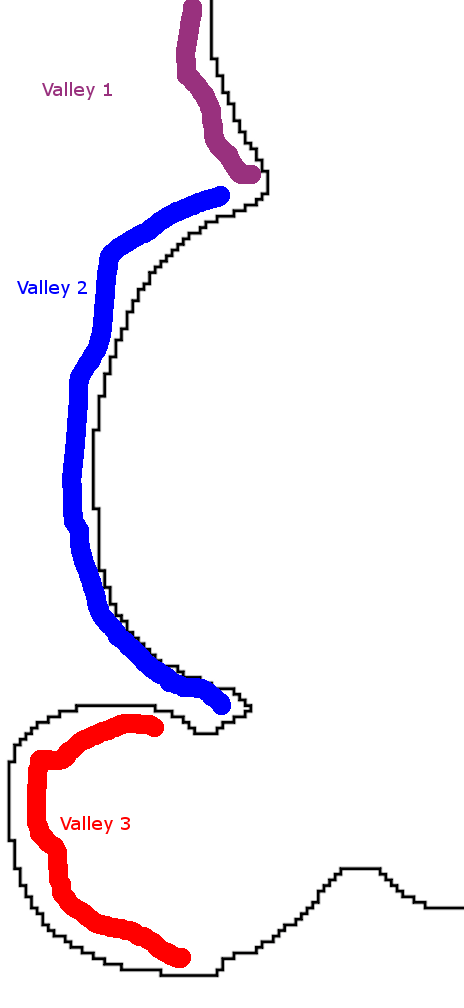
\includegraphics[width = 0.2\textwidth]{Figures/valleys}
%   \caption{Illustration of valleys. Valleys are defined for same pair of patches and each valley could contain at most one fold line.}
%   \label{fig:valley}
% \end{figure}


% In the next stage, the competition is among fold lines between same pair of segments with different direction. The intuition here is for some segment pairs, we are certain that which one should appear left (right), and we want to remove the fold line which indicates opposite direction. The process is conducted by checking two fold line between same segment pair but with different direction. If they can reach each other by going up or down along the segment boundary, we remove the one with lower score.

% After the filtering process, initial fold lines are already pretty nice. We further remove some fold lines if they are too close to some other fold lines with higher score. And for background segment, we only use one fold line candidate.

\subsection{Find Region Fold Line Candidates} \label{split_fold_line_candidates}
Intersection fold lines connect segments and make the popup craft more appealing and stable, but often it is necessary to add fold lines inside segments to make the popup craft foldable. We call these fold lines ``split fold lines''. As a split fold line splits a segment into halves, it also splits intersection fold lines of this segment into two groups. In this sense, a split fold line changes the topology of intersection fold lines. Appearing at different locations inside the segment, a split fold line changes the topology in different ways. In this manner, we divide the segment into multiple regions, each of which contains a split fold line candidate.

% Although most fold lines lie on the intersection between segment pairs, some segments themselves have to be folded to make the popup craft foldable (e.g. the fold lines on the arm of the bear example). A segment can be folded for arbitrary number of times at arbitrary position inside the segment. Similar with finding intersection fold line candidates, we divided the segment into multiple regions and associate one fold line candidate with each region. A fold line folds a segment into two halves, and at the same time, divides intersection fold line candidates into two groups. A region is defined such that whereever a fold line is put in the region, the division of intersection fold line candidates does not change. Then it is reasonable to add only one fold line candidate in each region and allows it to appear at any position in the region.

% After finding all initial fold lines, we can define the topology of initial fold lines on each segment. Here we look at the topology for each segment independently because a new fold line candidate only affect one segment. For segment $s$, we define the topology simply based on the connectivity of its initial fold lines on $R(s)$. We separate $R(s)$ into sub-regions in a sense that the topology is the same whereever a new fold line is put in the sub-region. We put a new fold line candidate in each sub-region (not for the ones which has no initial fold lines on its left or right).

\subsection{Structure and Properties} \label{popup_graph_structure}
%A segment-based popup graph has \textit{segments} as nodes and \textit{intersection fold line candidates} as edges connecting two segments. A segment-based popup graph has the following properties:

%\textbf{Background Enclosing: } A popup graph has a background segment enclosing all other segments.

%\textbf{Directed Acyclic Graph (DAG): } We denote the direction of an edge (fold line candidate) as from its left segment to its right segment. Then the graph excluding the background segment is a DAG.

%\textbf{Source and Sink: } The background segment serves as both the source and the sink for all paths.

A popup graph has fold line candidates as nodes, and their neighboring relations as edges. Two fold lines are regarded as neighbors only when they belong to the same segment and there is no fold line between them. A popup graph has the following properties:

\textbf{Background Enclosing: } The background segment has one split fold line candidate called \textit{background fold line} which is always active. The \textit{background fold line} divides the background segment into two halves. We call these two halves \textit{left background patch} and \textit{right background patch}. This corresponds to the two halves of most blessing cards.  We add two split fold lines at left and right image border to simplify notation. Then the left image border fold line is the source of the graph and the right image border fold line is the sink of the graph.

\textbf{Directed Acyclic Graph (DAG): } The left-right orientation between fold line candidate pairs is well-defined and the the graph excluding the background fold line is also a DAG.


% \subsection{Retrieve Popup Graph Information} \label{popup_graph_information}
% We can define the graph based on all fold line candidates. A fold line neighbor pair $(f_l, f_r)$ is found by looking at neighbor pixels. (Note that each fold line candidate occupies a region $R(f)$ on the image domain.) For $f_s$ and $f_t$ belonging to the same segment $s$, a fold line path $P(f_s, f_t)$ is defined as the sequence of fold lines of $s$ through which might affect the connectivity of $f_s$ and $f_t$. (See figure \ref{fig:path}.)

% \begin{figure}[h]
%   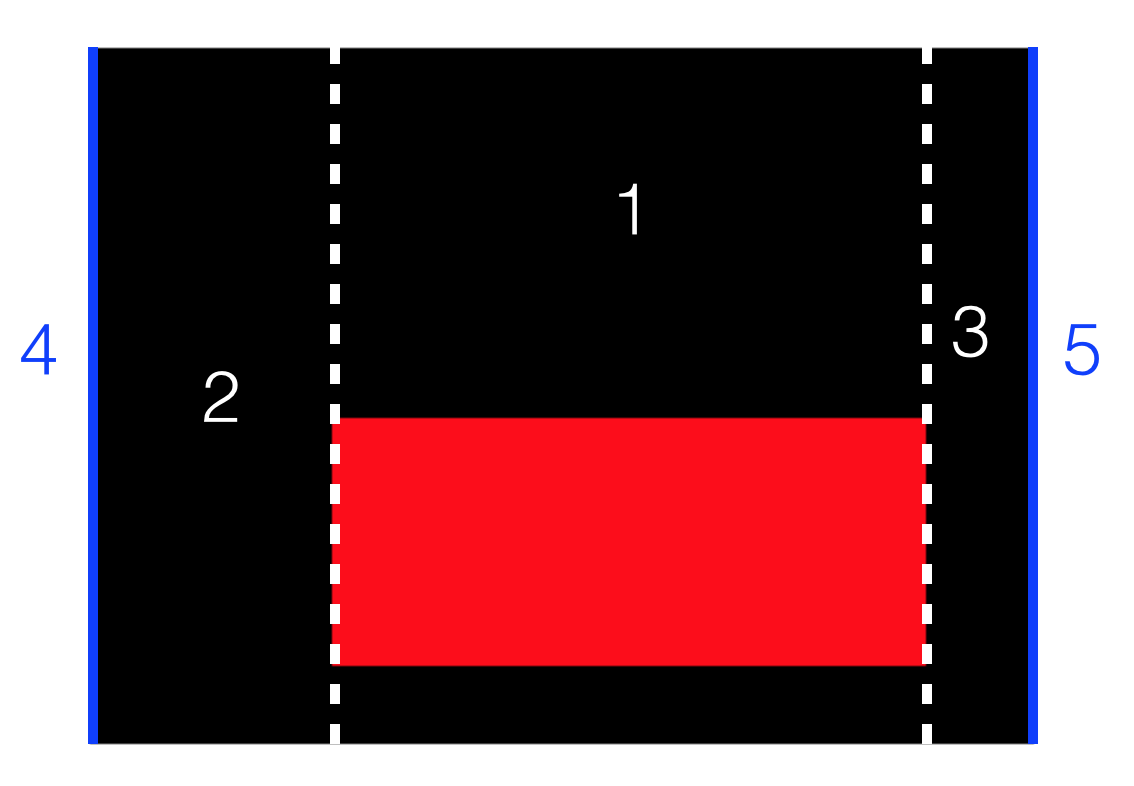
\includegraphics[width = 0.3\textwidth]{Figures/path}
%   \caption{We say fold line sequence \{2, 1, 3\} is a path between fold line 4 and fold line 5. Fold line 4 and fold line 5 will appear on the same final patch if fold line \{2, 1, 3\} are all inactive.}
%   \label{fig:path}
% \end{figure}


% We add two special fold lines, one for left image border $Lf$ and one for right image border $Rf$, to ease formulation.

